\documentclass[aspectratio=169]{beamer}
\usepackage[english]{babel}
\usepackage[utf8]{inputenc}
\usepackage{verbatim}
\usepackage{graphicx}
\usepackage{pgfpages}
\usepackage{ulem}
\usepackage{float}
\usepackage{amsmath}

\setbeameroption{hide notes}

\setbeamercolor{title}{fg=white}
\setbeamercolor{author}{fg=white}
\setbeamercolor{normal text}{fg=black}
\setbeamercolor{frametitle}{fg=black}
\setbeamercolor{item}{fg=red}
\setbeamercolor{block title}{fg=red}
\setbeamercolor{section in toc}{fg=red}
\setbeamercolor{footline}{fg=white}
\setbeamercolor{title in head/foot}{fg=white,bg=black}

\setbeamertemplate{navigation symbols}{}
\setbeamertemplate{headline}{
    
\includegraphics[height=1mm, width=\paperwidth]{wg-headline.png}
}

\setbeamertemplate{footline}{
    \begin{beamercolorbox}[ht=1.2em]{title in head/foot}
        {\footnotesize \hspace{1em}\inserttitle, \insertshortauthor}
    \end{beamercolorbox}
}

\begin{document}

\title{LinuxCon Europe 2013}
\author{Maksim Melnikau}
\date{}

{
\title{
    
\includegraphics[width=0.4\textwidth]{wg-logo.png}
    \\
    {\huge LinuxCon Europe 2013}
    \\
}

\usebackgroundtemplate{
\includegraphics[width=\paperwidth]{wg-end.jpg}}
\begin{frame}[plain]{}
    \titlepage
\end{frame}
}

\usebackgroundtemplate{
\includegraphics[width=\paperwidth]{wg-bg.jpg}}
\logo{
    
\includegraphics[height=1.7cm]{wg-logo.png}
}

{
\usebackgroundtemplate{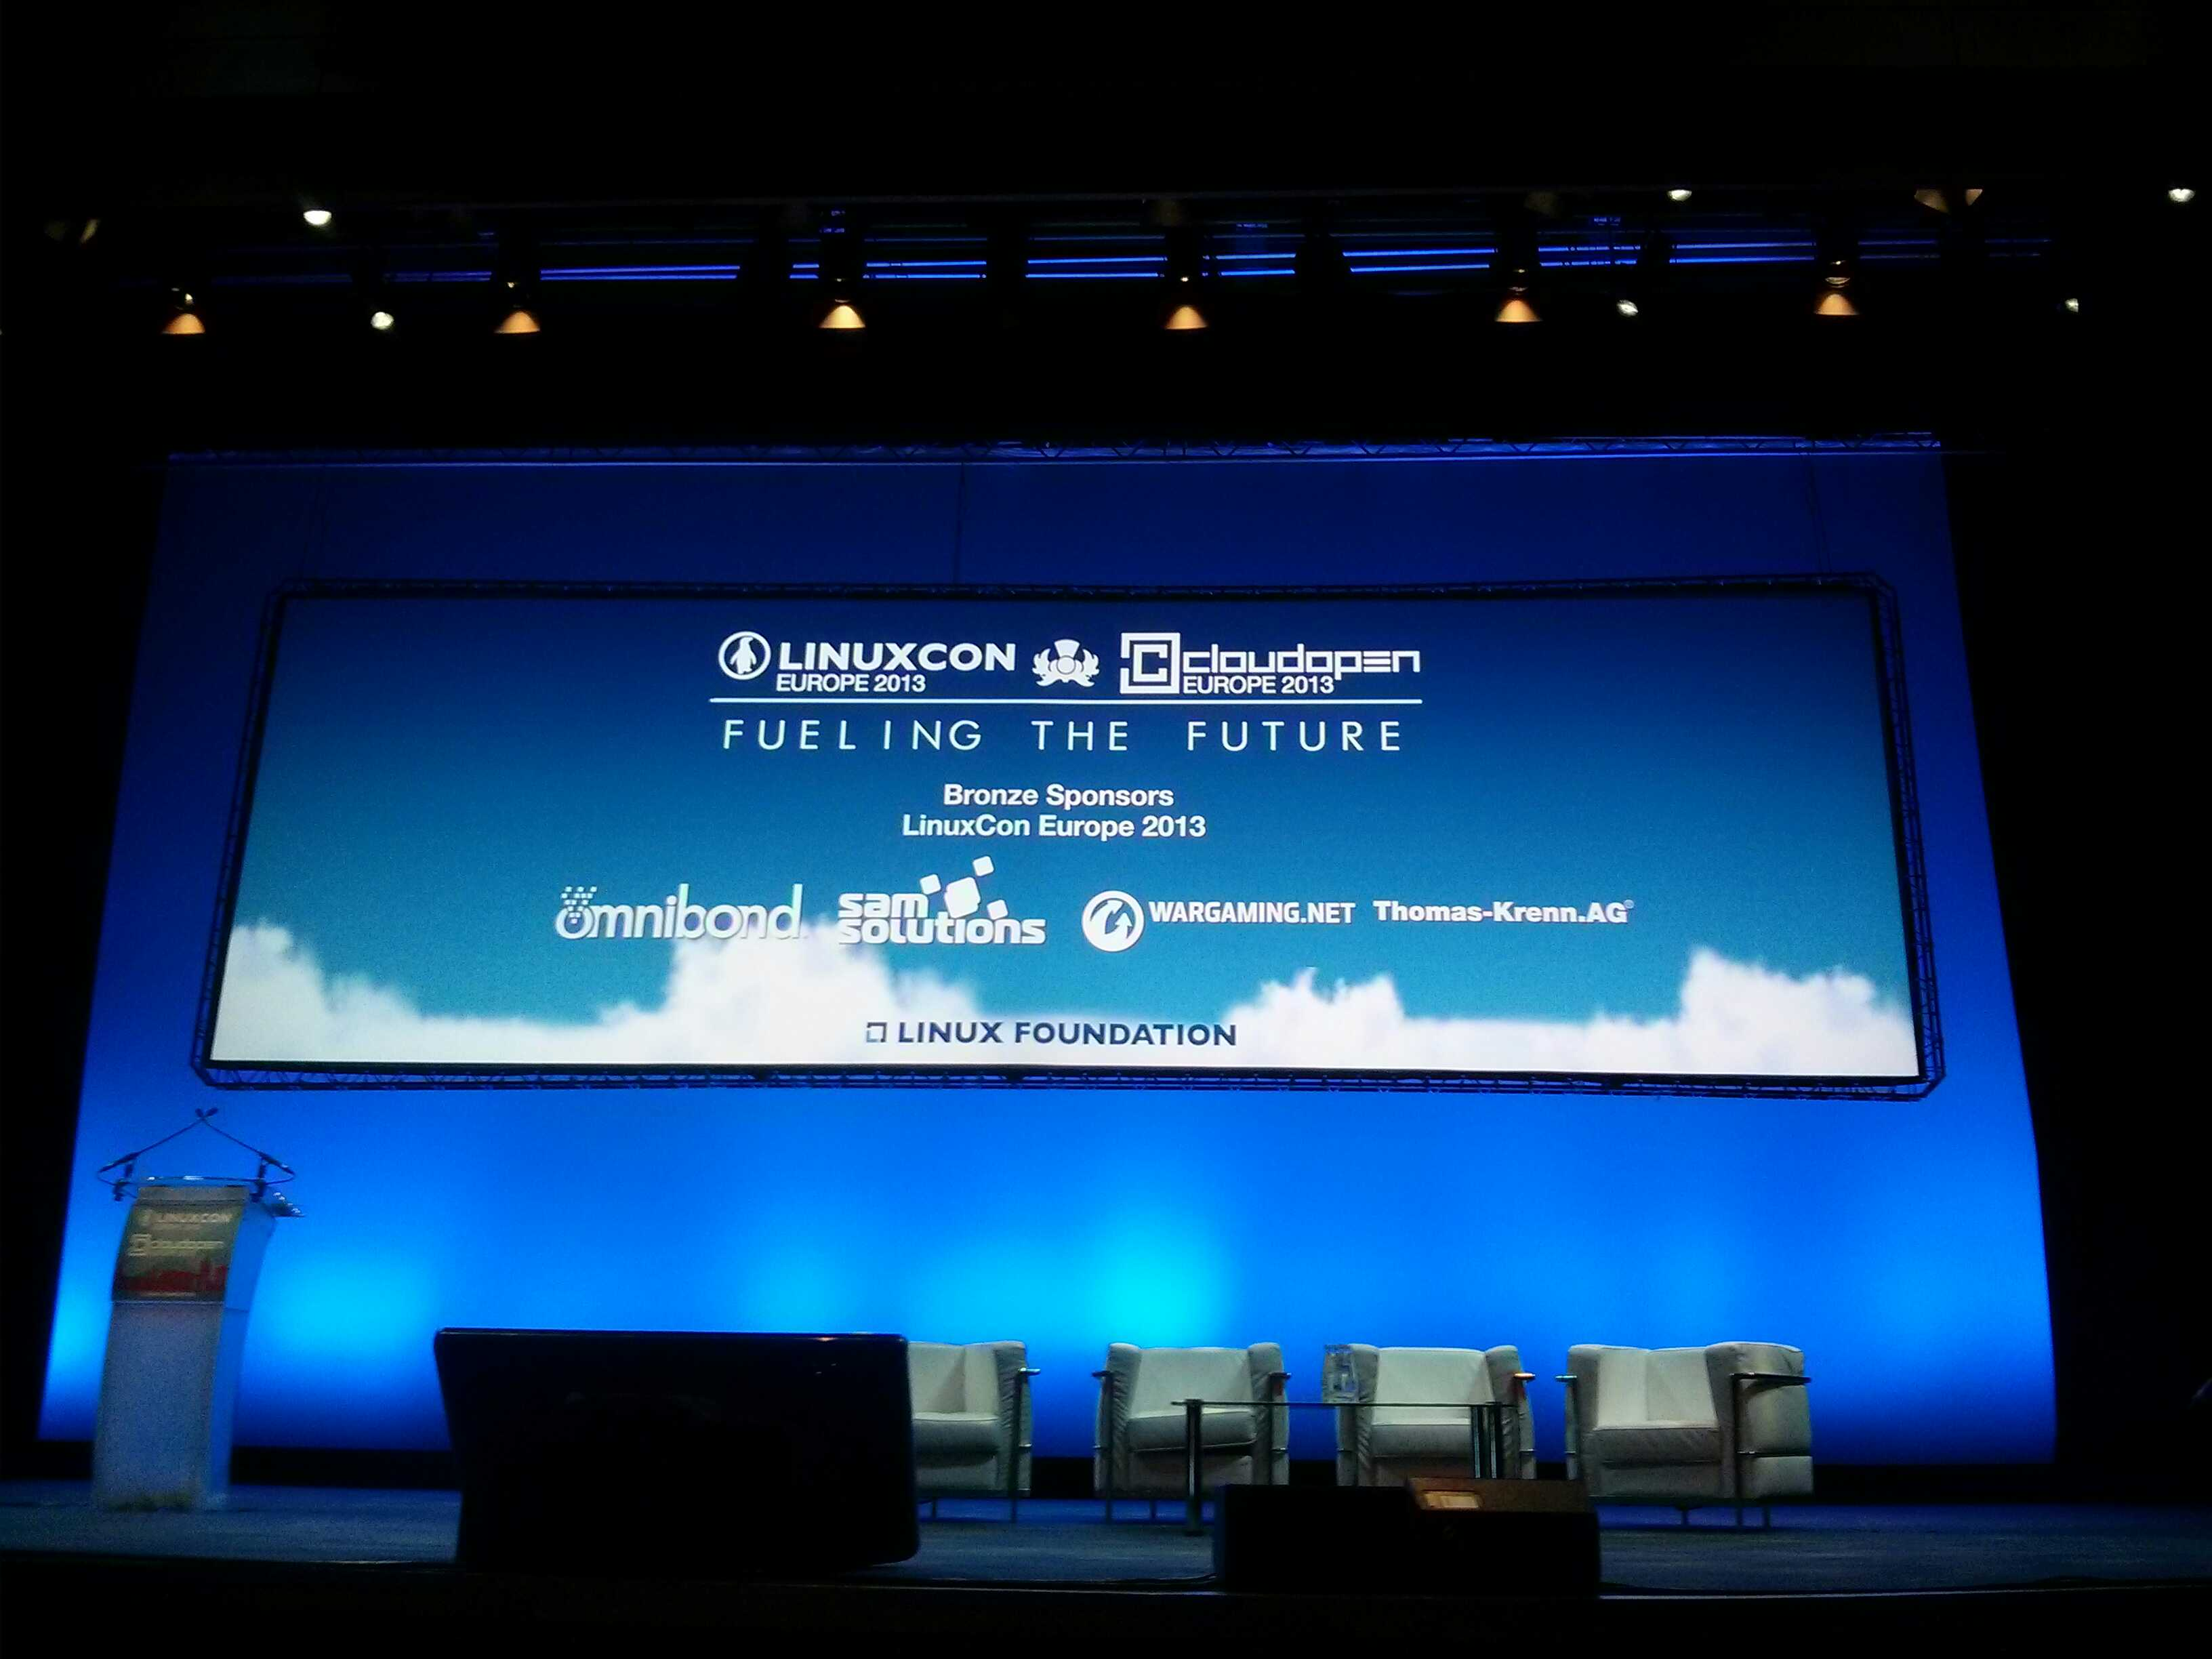
\includegraphics[width=\paperwidth]{sponsors.jpg}}
\begin{frame}[plain]{}
\end{frame}
}

\begin{frame}{Intro, Jim Zemlin}
  \begin{itemize}
  \item Xen and KVM under the same roof after so many years
  \item best way to use Linux - is via collaborate development
  \item twitter has 100 public repos on github
  \item for every \$1 spent on AWS, up to \$4 not being spent on traditional IT
  \item 1B html5 capable browsers, 2M web developers writing apps
  \item gaming industry towards Linux and Open Source
  \item huge talent war for developers
  \item we need more lawyers who understand open source and collaboration.
  \item Linux Foundation: some sponsors here only to recruit
  \item Linux - code as poetry, better, faster, cheaper.
  \end{itemize}
\end{frame}

\begin{frame}{We won, what next?, Mark Hinkle, Citrix}
  \begin{itemize}
  \item collaboration models are cool - being used in new \& different domains.
  \item FOSS sharing model will be adopted by governments \& helsthcareg
  \item Linux is running supercomputers, smartphones etc
  \item oss not a zero-sum game - companies add value on top of it.
  \item taking Linux and oss tols and finding ways to innovate in different categories.
  \item CERN LHC creates 30 petabytes of data a year
  \item Linux and OSS devs are setting the standard for the way tech will be developed
  \item Linux - platform for innovation
  \item let opensource culture be a lesson not just for software .... The future is open
  \item using oss to solve problems other domains: medicine, energy, etc
  \item the future is open and it's our responsibility to share what we know
  \end{itemize}
\end{frame}

\begin{frame}{Evolution Of The Twitter Stack, Chris Aniszczyk}
  \begin{itemize}
  \item 500M tweets a day, 6k tweets a second, 145k tps in peak
  \item failure is an option
  \item "throwing machines on problem" isn't the best solution, twitter at LinuxCon
  \item Twitter is of course all running on Linux, why would you need anything else?
  \item Twitter find solution for their problem - JVM
  \item zipkin - gives you a visual representation where most of the time fulfill in request
  \item Mesos, Linux and cgroups - reshare cluster dinamically
  \item twitter have 2000+ employees, half of them are engineers
  \item Embrace open source, Incremental change, Data center as computer
  \end{itemize}
\end{frame}

\begin{frame}{Application Level Tracing and Debugging Tools}
  \begin{itemize}
  \item gdb, valgrind - fine, but no overview and can change app behavior
  \item undo takes snapshots and you can run your program backwards
  \item strace, ltrace - solve some problems, but don't cope well with large applications
  \item LD\_PRELOAD - powerful interface that can trace and control application
  \item yocto project uses LD\_PRELOAD tool called PSeudo ('sudo') to fake root access
  \item glibc can have multiple version of same function
  \item multi machine jobs, suspend/resume, virtualization, one VM per app
  \item tracing problems - heterogeneous usecase, what to measure
  \item we all know about Design For Test - what about Design For Profiling ?!
  \item Big Data - monitoring everything and correlate
  \item difficult to get fine-grain coverage without harming performance
  \item cloud computing makes profiling even more complex
  \item LTTng - nice tracing solution for Linux
  \end{itemize}
\end{frame}

\begin{frame}{Architectural Changes in NetworkManager, Pavel Simerda}
  \begin{itemize}
  \item NM is about changing configuration on-the-fly and making notification
  \item NM was redesigned for server: use cases, making desktop behavior more optimal
  \item interesting question: what should be done, when NetworkManager restarts?
  \item NM runtime configuration; ipv4/ipv6; DNS
  \item api and tools - a lot of abilities to configure your interfaces
  \item NM still have a lot of problems with ipv6, some kernel features still missing
  \end{itemize}
\end{frame}

\begin{frame}{Exploring The Dustier Corners of System Firmware, Matthew Garrett}
  \begin{itemize}
  \item firmware - vendor "policy", sometimes it is the only one difference between devices
  \item OS and firmware do same task, but kernel never knows what firmware do
  \item acpi 5.0 would help a bit to "speak" with firmware
  \item Physical Device Location - colour, location, shape, size, etc (removable in Linux)
  \item firmware could help to log kernel crashes (pstore)
  \item WMI - easiest call firmware from Windows, commonly used for vendor extensions
  \item reading specs ACPI and UEFI - not the most efficient techniques
  \item follow http://lwn.net/Articles/367630/
  \item specs are rarely written with Linux in mind
  \item every vendor has his own method to speak with firmware
  \item and future could be "web api" calls to BMC
  \item UEFI have a lot of interesting things
  \end{itemize}
\end{frame}

\begin{frame}{Grand Unification of ACPI-based device Hot-Plug, Rafael J. Wysocki}
  \begin{itemize}
  \item ACPI - rules for communication between platform firmware and the OS
  \item ACPI Machine Language (AML), ACPI Source Language (ASL), ACPI Namespace
  \item kernel speak with device directly (good) or via AML Interpreter (bad)
  \item ACPI Hot-Plug Notification Values - Bus Check, Device Check, Eject Request
  \item with ACPI hot-plug allows you to add/remove even CPU and Memory
  \end{itemize}
\end{frame}

\begin{frame}{Snapshots of Ram in oVirt}
  \begin{itemize}
  \item system checkpoint - disk snapshot + memory snapshot
  \item oVirt could reuse memory snapshots
  \item libvirt have interesting feature - preview snapshots
  \end{itemize}
\end{frame}

\begin{frame}{Next Generation Cloud Platforms, Mac Devine}
  \begin{itemize}
  \item we are API generation developers...
  \item there are so many new challenges and opportunities for IT and for developers
  \item a cloud service is only as good as its API
  \item cloud first mentality is starting to prevail. Developed and deploy at cloud speed.
  \item CEOs now identify technology as the most important external force
  \item don't afraid of mistakes, afraid of not learning on them
  \item big data optimized to be easy and fast accessable from softlayer
  \item simplicity wins. The easier to consume, the more likely it'll be consumed
  \end{itemize}
\end{frame}

\begin{frame}{LinuxCon Panel: What's the next generation cloud platform?}
  \begin{itemize}
  \item all about APIs: quality, management.
  \item the internet of things is a Pandora's box
  \item how to adapt to diff geos, create predictability and scalability.
  \end{itemize}
\end{frame}

\begin{frame}{Samsung R\&D Innovation with Open Source Development, Yannick Pellet}
  \begin{itemize}
  \item samsung is \#7 contributor in Linux kernel development
  \item consumer --- collaborator --- contributor --- leadership and innovation
  \item in past 5 yrs Samsung: consumer --- big contributor
  \item not only combine open source and commercial products, but also do education
  \end{itemize}
\end{frame}

\begin{frame}{Linux Kernel Developer Panel}
  \begin{itemize}
  \item no separate scheduler per arch, even for arm
  \item all the work that enterprise systems did has helped embedded
  \item kernel developers put private emails directly to /dev/null, write to maillists
  \item how to get started? Ask specific questions. Always ask on the list.
  \item if you submit code, be around to maintain it
  \item device-tree is still flame topic in arm world
  \item on security: if you report a problem we'll fix it ASAP
  \item there will always be fixes. Linux changes because the world changes.
  \item how do you get better? Reading code is a really good way to learn.
  \end{itemize}
\end{frame}

\begin{frame}{systemd nspawn, Lennart Poettering}
  \begin{itemize}
  \item systemd-nspawn was written originally for testing purpose
  \item most distros have "one line" command to bootstrap os image
  \item and nspawn could run it "next line"
  \item systemd-nspawn demo goes successfully, but one small bug onhided
  \item machinectl - management interface to nspawn and other cgroups virtualizations
  \item there are still few bugs in linux kernel. systemd, fedora...
  \end{itemize}
\end{frame}

\begin{frame}{Linus Torvalds (and Dirk Hohndel)}
  \begin{itemize}
  \item Linus is happy that few latest linux kernel releases hadn't big problems
  \item the most important thing in maintainer, not tech skills, but responsibility
  \item good thing about technology --- when you do something wrong you can fix it 
  \item I use Open Source because it's fun and it works!
  \item I do Linux because I want to see it work on a desktop.
  \item the core kernel is solid. The new and exciting ideas are on the periphery.
  \item Linus Torvalds: If it gets boring or I can't cope, I'll retire.
  \item there's no end plan. What works is what survives.
  \item 10 Best Quotes from Linus Torvalds' Keynote http://bit.ly/18JYuqJ 
  \end{itemize}
\end{frame}

\begin{frame}{Living in a Surveillance State, Mikko Hypponen}
  \begin{itemize}
  \item wholesale blanket surveillance, on everyone.
  \item some surveillance is ok
  \item today, data is cheap, we can keep everything
  \item people are more honest with their search engine
  \item the Internet has become a colony of the United States.
  \item countries could fight with US services together - doing Open Source
  \item to fight these problems, use open source. Let's work together
  \end{itemize}
\end{frame}

\begin{frame}{Multi-layered Web Security, Konstantin Ryabitsev}
  \begin{itemize}
  \item why multiple layers - we are all made out of meat, fail gracefully
  \item encryption is easy to get wrong
  \item personal questions are backdoors to your system
  \item captchas help again bots (a bit), but expiring token help better
  \item templating system are just bad, keep an eye
  \item SELinux is first and foremost a labeling system
  \item ModSecurity - Web Application Firewall - analysis of http traffic
  \item but ModSecurity is not a silver bullet, and it even more complex than SELinux...
  \item most "vulnerability scanners" will only check well known software and bugs
  \item security trade-off in terms of: effort, money, usability
  \item be prepared when things fail
  \end{itemize}
\end{frame}

\begin{frame}{Qt Project 2 Years Later, Thiago Macieira}
  \begin{itemize}
  \item Qt has long line to openness, from QPL till GPLv3
  \item Qt openness motivation: desire to really be an open project
  \item Qt goals: one workflow for everyone, regardless of employer
  \item Qt project principles: Fair, Transparent, Inclusive, Meritocratic
  \item qt3d and qtwayland will be merged to qt some day
  \item Qt - 450 commits/week
  \item 75\% of qt contributions comes from digia now
  \item loss after nokia changes was quite big - about 25\%
  \item face-to-face meeting really helps broke the ice
  \end{itemize}
\end{frame}

\begin{frame}{OSv, Glauber Costa, Avi Kivity}
  \begin{itemize}
  \item app | app server | jvm | OS | hypervisor | OS | hardware
  \item jvm, operation system, hypervizor - do same job, wtf?!
  \item people don't update OS in VM now
  \item no hardware, no users, no apps --- most features not used
  \item OSv mission - be the best OS powering virtual machines in the cloud
  \item OSv runs application in kernel space! and api not changed for the app
  \item Be the best OS powering virtual machine in the cloud
  \item hypervizor OS has nice feature - you don't need to write so much drivers
  \item memcached runs 40\% better on OSv than native - I want check it myself!
  \item credibility --- open source these days
  \item OSv runs on kvm, xen hvm (still work in progress), vmware - planned
  \item virtio-app - bypass I/O stack completely - consume data from virtio rings
  \item virtualization 2.0 - stateless servers
  \item OSv could run your C apps*
  \end{itemize}
\end{frame}

\begin{frame}{Containers and the Cloud, James Bottomley}
  \begin{itemize}
  \item virtualization was so much hyped in 2005
  \item the enterprise charged down the Hypervisor alley
  \item the Hosting market turned to Containers
  \item concontainers - its all about density
  \item containers vs hypervisors - you know everything about it
  \item may be someday containers tools will be merged
  \end{itemize}
\end{frame}

\begin{frame}{GlusterFS Workshop}
  \begin{itemize}
  \item distributed storage system - see also: ceph, xtreamfs, fhgfs, glusterfs
  \item user space, global namespace, stackable, everything is file
  \item glusterfs clients - fuse, NFSv3 and Libgfapi for kvm, samba
  \item no metadata server, multi-protocol access, replication, self-healing
  \item is the simplest distribution fs in terms of setting env
  \item mainly for non-structured data - media, shared storage, big data, objects
  \item glusterfs could be nicely integrated to openstack
  \item distributed block storage for VM
  \item paradigm changes block --- object, central --- distributed, server --- storage
  \end{itemize}
\end{frame}

{
\setbeamertemplate{footline}{}
\setbeamercolor{frametitle}{fg=white}
\setbeamercolor{normal text}{fg=white}
\setbeamercolor{block title}{fg=white}
\setbeamercolor{block body}{fg=red}

\usebackgroundtemplate{
\includegraphics[height=\paperheight]{wg-end.jpg}}
\begin{frame}{Thank You. Questions}
    \begin{block}{Maksim Melnikau}
    \par \url{mailto:m\_melnikau@wargaming.net}
    \par \url{https://plus.google.com/114669104565190507739/}
    \par \url{https://twitter.com/max\_posedon}
    \par \url{http://wargaming.com}
    \end{block}
\end{frame}
}

\end{document}
